%%%%%%%%%%%%%%%%%%%%%%%%%%%%%%%%%%%%%%%%%
% Beamer Presentation
% LaTeX Template
% Version 1.0 (10/11/12)
%
% This template has been downloaded from:
% http://www.LaTeXTemplates.com
%
% License:
% CC BY-NC-SA 3.0 (http://creativecommons.org/licenses/by-nc-sa/3.0/)
%
%%%%%%%%%%%%%%%%%%%%%%%%%%%%%%%%%%%%%%%%%

%----------------------------------------------------------------------------------------
%	PACKAGES AND THEMES
%----------------------------------------------------------------------------------------

\documentclass{beamer}

\mode<presentation> {

% The Beamer class comes with a number of default slide themes
% which change the colors and layouts of slides. Below this is a list
% of all the themes, uncomment each in turn to see what they look like.

%\usetheme{default}
%\usetheme{AnnArbor}
%\usetheme{Antibes}
%\usetheme{Bergen}
%\usetheme{Berkeley}
%\usetheme{Berlin}
%\usetheme{Boadilla}
%\usetheme{CambridgeUS}
%\usetheme{Copenhagen}
%\usetheme{Darmstadt}
%\usetheme{Dresden}
%\usetheme{Frankfurt}
%\usetheme{Goettingen}
%\usetheme{Hannover}
%\usetheme{Ilmenau}
%\usetheme{JuanLesPins}
%\usetheme{Luebeck}
\usetheme{Madrid}
%\usetheme{Malmoe}
%\usetheme{Marburg}
%\usetheme{Montpellier}
%\usetheme{PaloAlto}
%\usetheme{Pittsburgh}
%\usetheme{Rochester}
%\usetheme{Singapore}
%\usetheme{Szeged}
%\usetheme{Warsaw}
\AtBeginSection[]
{
    \begin{frame}<beamer>
    \frametitle{}
    \tableofcontents[currentsection]
    \end{frame}
}
% As well as themes, the Beamer class has a number of color themes
% for any slide theme. Uncomment each of these in turn to see how it
% changes the colors of your current slide theme.

%\usecolortheme{albatross}
%\usecolortheme{beaver}
%\usecolortheme{beetle}
%\usecolortheme{crane}
%\usecolortheme{dolphin}
%\usecolortheme{dove}
%\usecolortheme{fly}
%\usecolortheme{lily}
%\usecolortheme{orchid}
%\usecolortheme{rose}
%\usecolortheme{seagull}
%\usecolortheme{seahorse}
%\usecolortheme{whale}
%\usecolortheme{wolverine}

%\setbeamertemplate{footline} % To remove the footer line in all slides uncomment this line
%\setbeamertemplate{footline}[page number] % To replace the footer line in all slides with a simple slide count uncomment this line

%\setbeamertemplate{navigation symbols}{} % To remove the navigation symbols from the bottom of all slides uncomment this line
}

\usepackage{amsmath}        % extensions for typesetting of math
\usepackage{amsfonts}       % math fonts
\usepackage{amsthm}         % theorems, definitions, etc.
\usepackage{amssymb}
\usepackage{bbding}         % various symbols (squares, asterisks, scissors, ...)
\usepackage{bm}             % boldface symbols (\bm)
\usepackage{caption}
\usepackage[aboveskip=2pt]{subcaption}
\usepackage{graphicx} % Allows including images
\usepackage{booktabs} % Allows the use of \toprule, \midrule and \bottomrule in tables
\usepackage{natbib}         % citation style AUTHOR (YEAR), or AUTHOR [NUMBER]

\usepackage[linguistics]{forest}
\forestset{
dg edges/.style={for tree={parent anchor=south, child anchor=north,align=center,base=bottom,where n children=0{tier=word,edge=dotted,calign with current edge}{}}},
}
\usepackage[noabbrev,capitalise]{cleveref}
\usepackage{tikz-dependency}
\usepackage{pgfplots}
\pgfplotsset{compat=1.15}
\usepackage{xspace}

\def\de2cs{\texttt{de2cs}\xspace}
\def\cs2en{\texttt{cs2en}\xspace}
\def\transformer{Transformer\xspace}
\def\transformerbase{\texttt{Transformer base}\xspace}
\def\transformerrel{\texttt{Transformer relative}\xspace}
\def\seq2seq{\texttt{seq2seq}\xspace}
\def\DiagonalParse{\texttt{DiagonalParse}\xspace}
\def\DepParse{\texttt{DepParse}\xspace}
\def\TreeDistance{\texttt{TreeDistance}\xspace}
\def\TreeTraversal{\texttt{TreeTraversal}\xspace}
\def\SpecPOS{\texttt{SpecPOS}\xspace}
\def\SpecDep{\texttt{SpecDep}\xspace}
%----------------------------------------------------------------------------------------
%	TITLE PAGE
%----------------------------------------------------------------------------------------

\title[Exploiting Sentence Structure in NMT]{Exploiting Sentence Structure in\\Neural Machine Translation} % The short title appears at the bottom of every slide, the full title is only on the title page

\author[Thuong-Hai Pham]{Thuong-Hai Pham\\
\medskip
\small{Supervisor: RNDr. Ond\v{r}ej Bojar, PhD}} % Your name
\institute[UFAL] % Your institution as it will appear on the bottom of every slide, may be shorthand to save space
{
Institute of Formal and Applied Linguistics\\
Faculty of Mathematics and Physics\\
Charles University \\ % Your institution for the title page
\medskip
\textit{pham@ufal.mff.cuni.cz} % Your email address
}
\date{\today} % Date, can be changed to a custom date

\begin{document}

\begin{frame}
\titlepage % Print the title page as the first slide
\end{frame}

%------------------------------------------------

\begin{frame}{Research Questions}
\begin{block}
1 Does feeding source-side syntactic knowledge to the Transformer \citep{DBLP:conf/nips/VaswaniSPUJGKP17} help translation quality?
\end{block}
\begin{block}
2 Is the attention mechanism perhaps already capturing this information?
\end{block}
\end{frame}

% \begin{frame}{Positional Embeddings}
% \begin{figure}
%     \centering
%     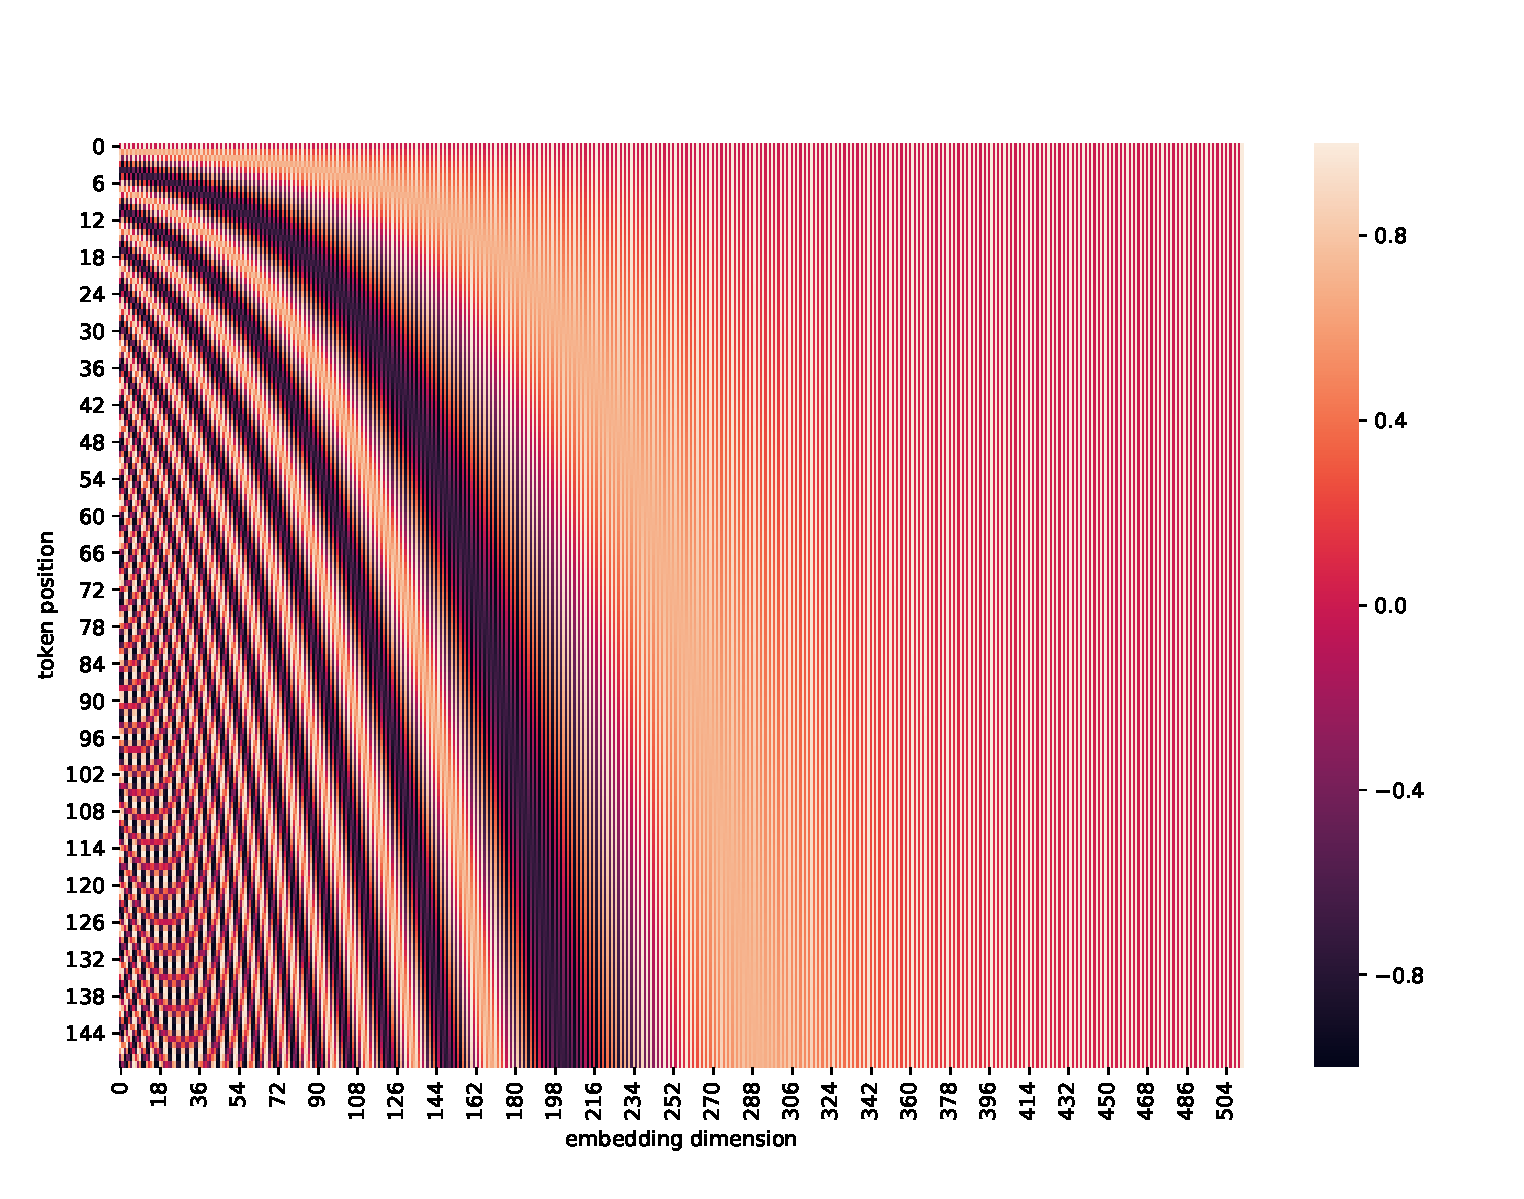
\includegraphics[width=\linewidth]{img/positional-embedding.pdf}
%     \caption{Positional embeddings with sine and cosine functions, embedding size $d=512$.}
%     \label{fig:positional-embedding}
% \end{figure}
% \end{frame}

%------------------------------------------------

\begin{frame}
\frametitle{Overview} % Table of contents slide, comment this block out to remove it
\tableofcontents % Throughout your presentation, if you choose to use \section{} and \subsection{} commands, these will automatically be printed on this slide as an overview of your presentation
\end{frame}

%----------------------------------------------------------------------------------------
%	PRESENTATION SLIDES
%----------------------------------------------------------------------------------------

%------------------------------------------------
\section{Enriching the Encoder by Targeting Self-Attention}
%------------------------------------------------
\subsection{Structured Attentional Bias}
%------------------------------------------------

\begin{frame}{Structured Attentional Bias}
\begin{itemize}
    \item Attention function in the \transformer
    \begin{equation}\label{eq:attf}
        e_{ij}=\frac{1}{\sqrt{d_k}} x_i W^Q (x_j W^K)^\top
    \end{equation}
    \item Relative position \citep{DBLP:conf/naacl/ShawUV18}
    \begin{equation}
        e_{ij}=\frac{1}{\sqrt{d_k}} x_i W^Q (x_j W^K + b^K_{ij})^\top
    \end{equation}
\end{itemize}
\begin{figure}[t]
    \centering
    \begin{dependency}
        \begin{deptext}
        I \& think \& this \& is \& a \& good \& idea \& . \\
        \end{deptext}
        \depedge{4}{1}{-3}
        \depedge{4}{2}{-2}
        \depedge{4}{3}{-1}
        \depedge{4}{5}{1}
        \depedge{4}{6}{2}
        \depedge{4}{7}{3}
        \depedge{4}{8}{4}
    \end{dependency}
\end{figure}
\end{frame}

%------------------------------------------------

\begin{frame}{Structured Attentional Bias - Tree Distance}

\begin{figure}[t]
    \centering
    \begin{forest}
    dg edges
    [ROOT
        [think, edge={<-}, edge label={node[midway,fill=white] {2}}
          [I, edge={->}, edge label={node[midway,fill=white] {2}} [I]] 
          [think]
          [\textbf{is}, red, edge={<-}, edge label={node[midway,fill=white] {1}}
          	[this, edge={->}, edge label={node[midway,fill=white] {1}} [this]]
            [is]
            [idea, edge={->}, edge label={node[midway,fill=white] {1}}
            	[a, edge={->}, edge label={node[midway,fill=white] {2}} [a]]
                [good, edge={->}, edge label={node[midway,fill=white] {2}} [good]]
                [idea]
            ]
          ]
        ]
        [., edge={->}, edge label={node[midway,fill=white] {3}} [.]]
    ]
    \end{forest}
\end{figure}

\end{frame}

%------------------------------------------------

\begin{frame}
\frametitle{Structured Attentional Bias - Tree Traversal Encoding}

\begin{figure}[t]
    \centering
    \begin{forest}
    dg edges
    [ROOT
        [think, edge={<-}, edge label={node[midway,fill=white] {UU}}
          [I, edge={->}, edge label={node[midway,fill=white] {L}} [I]] 
          [think]
          [\textbf{is}, red, edge={<-}, edge label={node[midway,fill=white] {U}}
          	[this, edge={->}, edge label={node[midway,fill=white] {D}} [this]]
            [is]
            [idea, edge={->}, edge label={node[midway,fill=white] {D}}
            	[a, edge={->}, edge label={node[midway,fill=white] {DD}} [a]]
                [good, edge={->} [good]]
                [idea]
            ]
          ]
        ]
        [., edge={->}, edge label={node[midway,fill=white] {UUD}} [.]]
    ]
    \end{forest}
\end{figure}
\end{frame}

%------------------------------------------------
\subsection{Specialized Attention Heads}
%------------------------------------------------

\begin{frame}{Specialized Attention Heads}
\begin{equation}\tag{\ref{eq:attf}}
    e_{ij}=\frac{1}{\sqrt{d_k}} x_i W^Q (x_j W^K)^\top
\end{equation}
\begin{figure}[t]
    \centering
    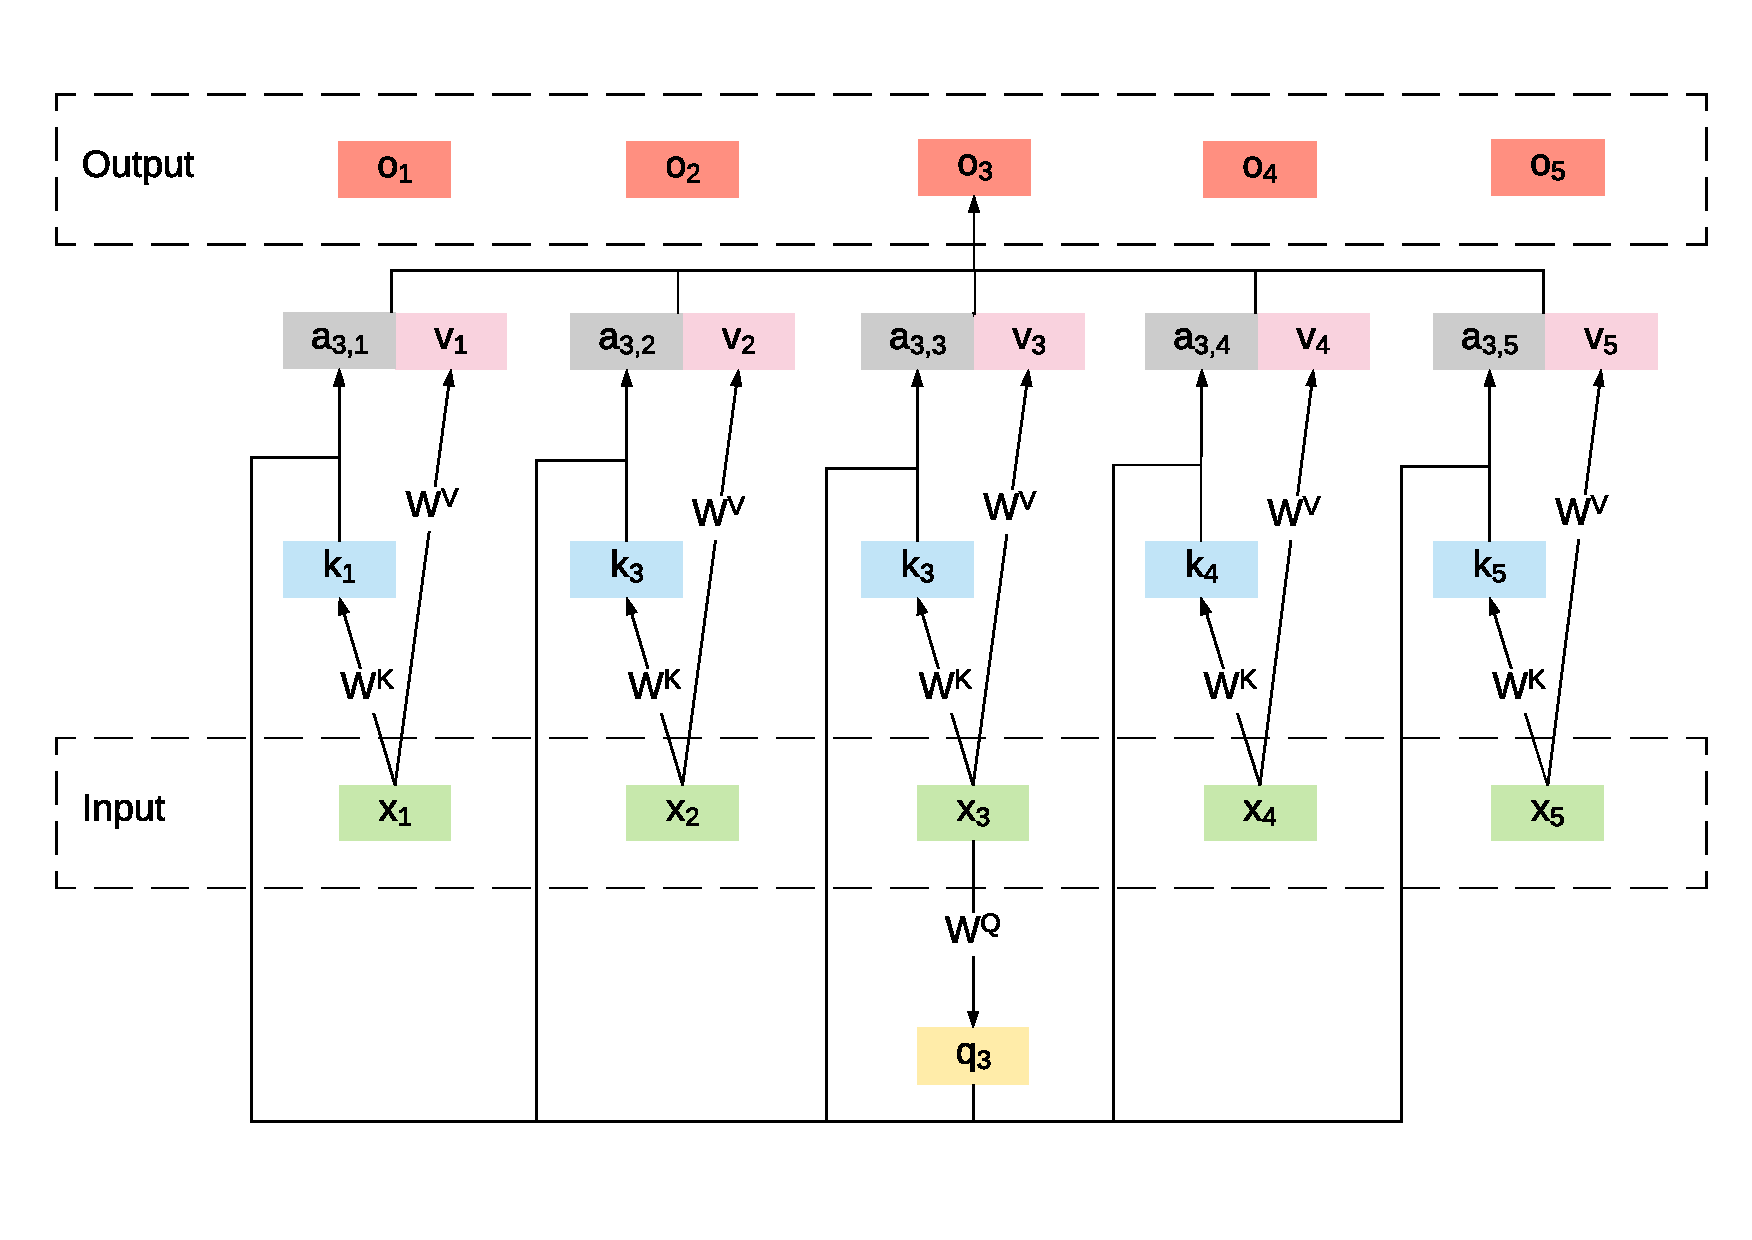
\includegraphics[width=0.7\linewidth]{img/self-att.pdf}
\end{figure}
\end{frame}

%------------------------------------------------

\begin{frame}{Specialized Attention Heads}
\begin{figure}[t]
    \centering
    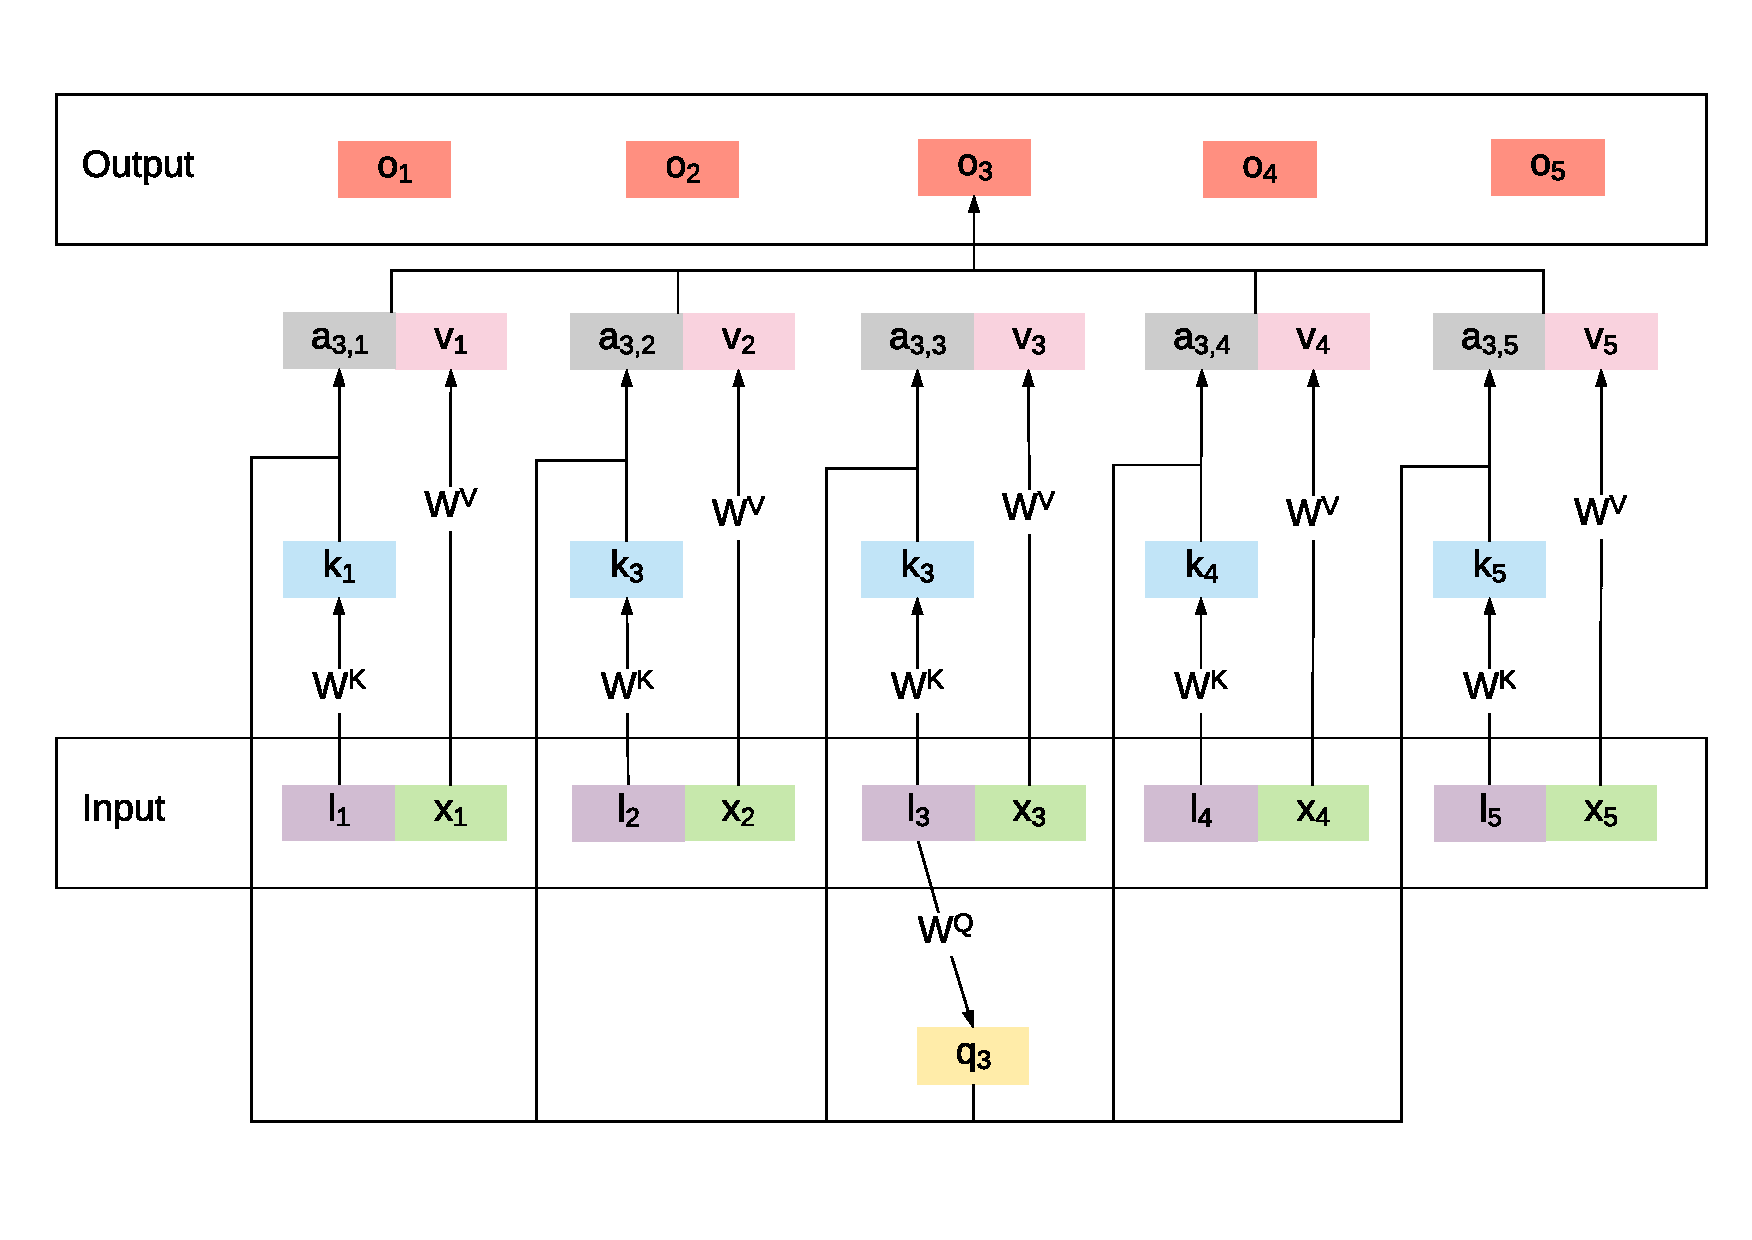
\includegraphics[width=0.7\linewidth]{img/specialized-head.pdf}
\end{figure}
\end{frame}

%------------------------------------------------
\subsection{Experiment Settings}
%------------------------------------------------

\begin{frame}{Experiment Settings}
\begin{itemize}
    \item \cs2en (5.2M sentence pairs, subset of CzEng 1.7 \citep{czeng16:2016}).
    \item Training for 500,000 steps with batch size 3072.
    \item Baselines
        \begin{itemize}
            \item \textbf{\transformerbase} - default hyperparameter set \textit{transformer\_base}.
            \item \textbf{\transformerrel} \citep{DBLP:conf/naacl/ShawUV18}.
        \end{itemize}
    \item Our models
    \begin{itemize}
        \item \textbf{\TreeDistance} - \transformer with tree distance.
        \item \textbf{\TreeTraversal} - \transformer with tree traversal.
        \item \textbf{\SpecPOS} - \transformer with specialized attention head guided by POS tags.
        \item \textbf{\SpecDep} - \transformer with specialized attention head guided by dependency labels.
    \end{itemize}
\end{itemize}
\end{frame}

%------------------------------------------------
\subsection{Results}
%------------------------------------------------

\begin{frame}{Results}
\begin{table}[t]
    \small
    \begin{center}
    \begin{tabular}{lcc}
        \textbf{Model}        	                            & \textbf{Dev}	& \textbf{Test}	\\
        \hline
        \transformerbase (base)    					        & 37.28 & 36.66 \\
        \transformerrel	(relative)				            & 37.23 & 37.02$^{\dag}$ \\
        \hline
        \TreeDistance				                        & 34.45 & 35.50 \\
        \TreeTraversal					                    & 35.21 & 35.80 \\
        (base) + \TreeDistance      					    & 37.67 & 37.49$^{\ddag\blacktriangledown}$ \\
        % (base) + tree distance, max 20					    &  &  \\
        % (base) + tree traversal					        &  &  \\
        (relative) + \TreeDistance      			        & 37.15 & 37.55$^{\ddag\blacktriangledown}$ \\
        (relative) + \TreeTraversal				            & 38.22 & \textbf{37.80}$^{\ddag\blacktriangledown}$ \\
        \hline
        (base) + \SpecPOS						& 36.97 & 36.65 \\
        (relative) + \SpecPOS			& 37.81 & 36.93$^{\dag}$ \\
        (base) + \SpecDep		& 37.53 &  37.72$^{\ddag\blacktriangledown}$ \\
        (relative) + \SpecDep		& 37.66 & \textbf{37.97}$^{\ddag\blacktriangledown}$  \\
    \end{tabular}
    \end{center}
\end{table}
\begin{itemize}
    \item \TreeDistance and \TreeTraversal showed no improvement on their on. When combining with sequential embeddings (base and relative), they reported +0.5 to +0.8 BLEU against both baselines.
    \item \SpecDep brought +0.95 to +1.06 compared against the baselines, while \SpecPOS did not.
    % \item  Statistical significance marked as $\dag$ ($p < 0.05$) and $\ddag$ ($p < 0.01$) when compared to \transformerbase and $\triangledown/\blacktriangledown$ when compared to \transformerrel.
\end{itemize}
\end{frame}

%------------------------------------------------
\section{Interpreting Self-Attention as Parse}
%------------------------------------------------

\begin{frame}{Dependency Parse}
\begin{figure}[t]
    \begin{minipage}[b]{0.50\linewidth}
        \centering
        \begin{dependency}[text only label]
            \begin{deptext}
            I \& shot \& an \& elephant \& in \& my \& pajamas \\
            \end{deptext}
            \depedge{2}{1}{}
            \depedge{2}{4}{}
            \depedge{4}{3}{}
            \depedge{4}{5}{}
            \depedge{5}{7}{}
            \depedge{7}{6}{}
        \end{dependency}
    % \rule{6cm}{6cm} %to simulate an actual figure
    \end{minipage}%
    \begin{minipage}[b]{0.50\linewidth}
        \centering
            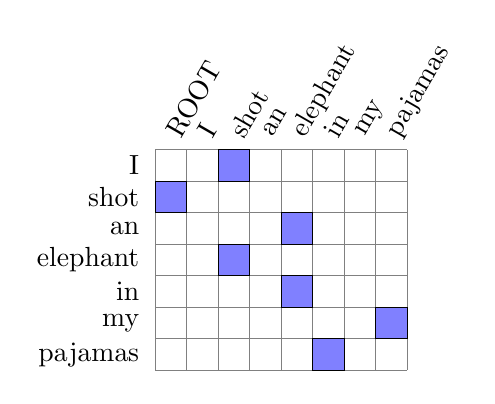
\begin{tikzpicture}[scale=0.4]
                \draw[step=1cm,draw=gray] (0,0) grid (8,7);
                
                \foreach \f [count=\y] in {I, shot, an, elephant, in, my, pajamas} {
                    \node[left] at (-.2,7.5-\y) {{\raggedleft \f }};
                }
                
                \foreach \e [count=\x] in {ROOT, I, shot, an, elephant, in, my, pajamas} {
                    \node[rotate=60,right] at (\x-.6,7.2) {{\raggedright \e}};
                }
                
                % draw word alignment
                \foreach \x [count=\y] in {2, 0, 4, 2, 4, 7, 5} {
                    \draw[fill=blue!50] (\x,7-\y) rectangle +(1,1);
                }
            \end{tikzpicture}
    \end{minipage}
    \label{fig:deptree-vs-matrix}
\end{figure}
A dependency tree and its representation as an adjacency matrix (the columns represent the heads, the rows are dependents).
\end{frame}

%------------------------------------------------
\subsection{Self-Attention as Dependency Parse}
%------------------------------------------------

\begin{frame}{Self-Attention as Dependency Parse}
    \begin{figure}[t]
    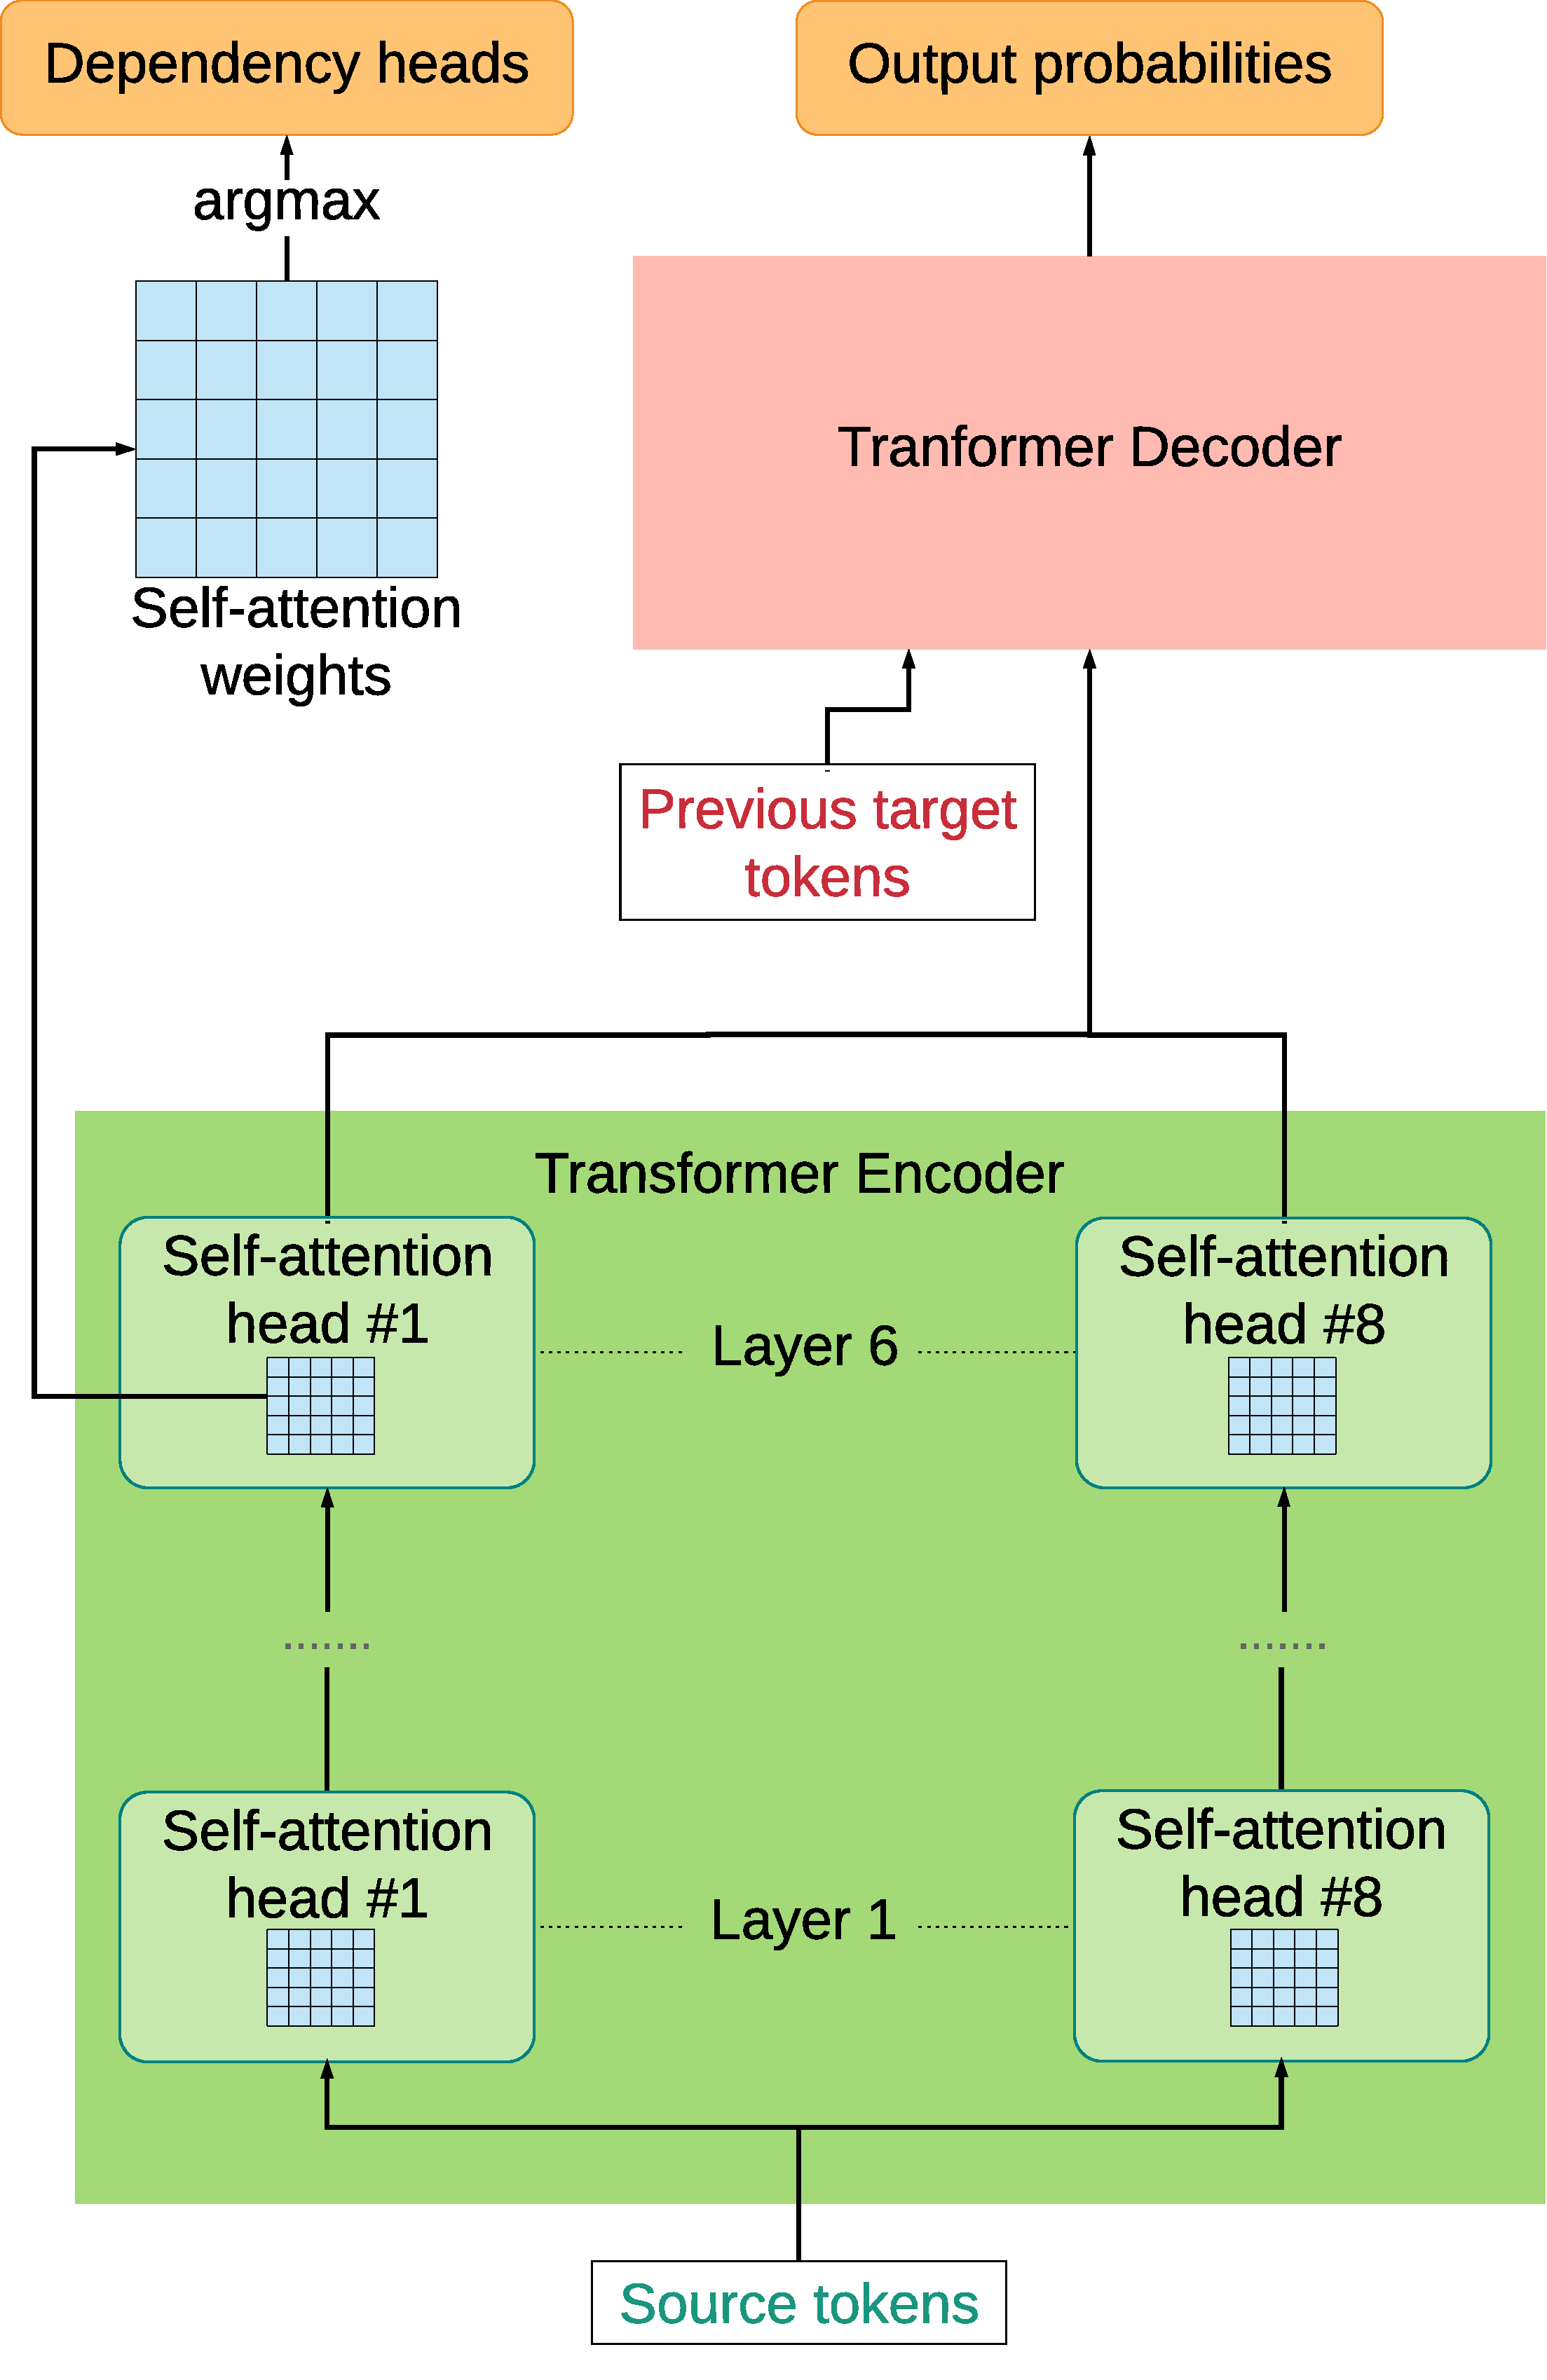
\includegraphics[width=0.43\textwidth]{img/joint_model_compated}
\end{figure}
\end{frame}

%------------------------------------------------
\subsection{Self-Attention as Diagonal Parse}
%------------------------------------------------

\begin{frame}{Self-Attention as Diagonal Parse}
\begin{figure}[t]
    \begin{minipage}[b]{0.50\linewidth}
        \centering
        \begin{dependency}[text only label]
            \begin{deptext}
            I \& shot \& an \& elephant \& in \& my \& pajamas \\
            \end{deptext}
            \depedge{1}{2}{}
            \depedge{2}{3}{}
            \depedge{3}{4}{}
            \depedge{4}{5}{}
            \depedge{5}{6}{}
            \depedge{6}{7}{}
        \end{dependency}
    % \rule{6cm}{6cm} %to simulate an actual figure
    \end{minipage}%
    \begin{minipage}[b]{0.50\linewidth}
        \centering
            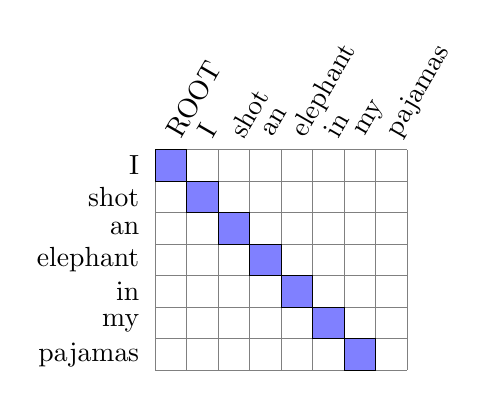
\begin{tikzpicture}[scale=0.4]
                \draw[step=1cm,draw=gray] (0,0) grid (8,7);
                
                \foreach \f [count=\y] in {I, shot, an, elephant, in, my, pajamas} {
                    \node[left] at (-.2,7.5-\y) {{\raggedleft \f }};
                }
                
                \foreach \e [count=\x] in {ROOT, I, shot, an, elephant, in, my, pajamas} {
                    \node[rotate=60,right] at (\x-.6,7.2) {{\raggedright \e}};
                }
                
                % draw word alignment
                \foreach \x [count=\y] in {0, 1, 2, 3, 4, 5, 6} {
                    \draw[fill=blue!50] (\x,7-\y) rectangle +(1,1);
                }
            \end{tikzpicture}
    \end{minipage}
\end{figure}
Dummy dependencies with diagonal matrix (the columns represent the heads, the rows are dependents).
\end{frame}

%------------------------------------------------
\subsection{Experiment Settings}
%------------------------------------------------

\begin{frame}{Experiment Settings}
    \begin{itemize}
        \item\cs2en datasets (PDT) and \de2cs \citep{machacek2018de2cs} (UD, 8.8M sentence pairs).
        \item Training for 500,000 steps with batch size 3072.
        \item Baseline: \transformerbase.
        \item Our models:
        \begin{itemize}
            \item \textbf{\DepParse} \& \textbf{\DiagonalParse} - Leveraging self-attention weights of the \transformer's encoder to jointly translate and parse source sentences.
            \item Each has 6 variants, i.e. from which layer the parse tree matrix is demanded: 0 to 5.
        \end{itemize}
    \end{itemize}
\end{frame}

%------------------------------------------------
\subsection{Results}
%------------------------------------------------

\begin{frame}{Results - \DepParse}
BLEU scores on test sets for translation task. Statistical significance marked as $\dag$ ($p < 0.05$) and $\ddag$ ($p < 0.01$) when compared to \transformerbase.
\begin{table}[t]
    \small
    \begin{center}
    \begin{tabular}{lcc}
        \textbf{Model}        	& \textbf{\de2cs}	& \textbf{\cs2en}	\\
        \hline
        \transformerbase    & 13.96	&  36.66 \\
        \DepParse		& 14.27$^\dag$	&  38.01$^\ddag$ \\
    \end{tabular}
    \end{center}
\end{table}

UAS on the gold-annotated test sets for parsing task.
\begin{table}[t]
    \small
    \begin{center}
    \begin{tabular}{lcc}
    \textbf{Model}        	& \textbf{de}	& \textbf{cs}	\\
    \hline
    % Stanford \citep{dozat-qi-manning:2017:K17-3} & 84.10 & -- \\
    UDPipe 1.2 (de) 		& 74.27 & -- \\ % UAS: 74.15, LAS: 68.61 in CoNLL Shared task 2017
    Nakagawa (2007) 		& -- &  86.28 \\
    \DepParse			& 81.23 	&  82.53 \\
    \end{tabular}
    \end{center}
    \label{multidec-results-parse}
\end{table}
\end{frame}

%------------------------------------------------

\begin{frame}{Results - \DepParse}
\begin{table}[t]
\small
\centering
\vspace{2ex}
  \begin{tabular}{lcc|cc}
    &  \multicolumn{2}{c}{\textbf{BLEU}} & \multicolumn{2}{|c}{\textbf{UAS}} \\
    & \textbf{Dev} & \textbf{Test} & \textbf{Dev} & \textbf{Test} \\
    \hline
    \transformerbase & 37.28 & 36.66 & -- & -- \\
    \hline
    Syntax demanded from head on layer 0 & 36.95 & 36.60 & 81.39 & 82.85 \\
    Syntax demanded from head on layer 1 & 38.51 & \textbf{38.01} & 90.17 & 90.78 \\
    Syntax demanded from head on layer 2 & 38.50 & 37.87 & 91.31 & 91.18 \\
    Syntax demanded from head on layer 3 & 38.37 & 37.67 & 91.43 & 91.43 \\
    Syntax demanded from head on layer 4 & 37.86 & 37.60 & 91.65 & \textbf{91.56} \\
    Syntax demanded from head on layer 5 & 37.63 & 37.67 & 91.44 & 91.46 \\
  \end{tabular}
\end{table}
\begin{itemize}
    \item Except layer 0, BLEU is higher when demanding syntax at shallower layer.
    \item UAS is better when demanding syntax at deeper layer.
    \item All test BLEU gains, except for layer 0, are statistically significant with $p<0.01$ when compared to \transformerbase.
\end{itemize}
\end{frame}

%------------------------------------------------

\begin{frame}{Results - \DiagonalParse}
\begin{table}[t]
\small
\centering
\vspace{2ex}
  \begin{tabular}{lcc|cc}
    &  \multicolumn{2}{c}{\textbf{BLEU}} & \multicolumn{2}{|c}{\textbf{Precision}} \\
    & \textbf{Dev} & \textbf{Test} & \textbf{Dev} & \textbf{Test} \\
    \hline
    \transformerbase & 37.28 & 36.66 & -- & -- \\
    \hline
    Syntax demanded from head on layer 0 & 38.68 & \textbf{38.14} & 99.97 & 99.96 \\
    Syntax demanded from head on layer 1 & 39.11 & 38.06 & 99.99 & \textbf{99.99} \\
    Syntax demanded from head on layer 2 & 37.85 & 37.85 & 99.98 & 99.98 \\
    Syntax demanded from head on layer 3 & 37.93 & 37.70 & 99.97 & 99.98 \\
    Syntax demanded from head on layer 4 & 37.68 & 37.47 & 99.98 & 99.96 \\
    Syntax demanded from head on layer 5 & 37.53 & 37.54 & 99.96 & 99.95 \\
  \end{tabular}
\end{table}
\begin{itemize}
    \item BLEU decreases when demanding syntax at higher layer.
    \item All test BLEU improvements are statistically significant with $p<0.01$ when compared to the \transformerbase.
\end{itemize}
\end{frame}

%------------------------------------------------

% \begin{frame}
% \frametitle{Blocks of Highlighted Text}
% \begin{block}{Block 1}
% Lorem ipsum dolor sit amet, consectetur adipiscing elit. Integer lectus nisl, ultricies in feugiat rutrum, porttitor sit amet augue. Aliquam ut tortor mauris. Sed volutpat ante purus, quis accumsan dolor.
% \end{block}

% \begin{block}{Block 2}
% Pellentesque sed tellus purus. Class aptent taciti sociosqu ad litora torquent per conubia nostra, per inceptos himenaeos. Vestibulum quis magna at risus dictum tempor eu vitae velit.
% \end{block}

% \begin{block}{Block 3}
% Suspendisse tincidunt sagittis gravida. Curabitur condimentum, enim sed venenatis rutrum, ipsum neque consectetur orci, sed blandit justo nisi ac lacus.
% \end{block}
% \end{frame}

%------------------------------------------------

% \begin{frame}
% \frametitle{Multiple Columns}
% \begin{columns}[c] % The "c" option specifies centered vertical alignment while the "t" option is used for top vertical alignment

% \column{.45\textwidth} % Left column and width
% \textbf{Heading}
% \begin{enumerate}
% \item Statement
% \item Explanation
% \item Example
% \end{enumerate}

% \column{.5\textwidth} % Right column and width
% Lorem ipsum dolor sit amet, consectetur adipiscing elit. Integer lectus nisl, ultricies in feugiat rutrum, porttitor sit amet augue. Aliquam ut tortor mauris. Sed volutpat ante purus, quis accumsan dolor.

% \end{columns}
% \end{frame}

%------------------------------------------------
\section{Conclusion \& Future Works}
%------------------------------------------------

\begin{frame}{Conclusion}
\begin{itemize}
    \item We proposed several methods to enrich and extract sentence structure from the attention mechanism in the Transformer model.
    
    \item Enriching the encoder with source-side dependency tree can help.
    \begin{itemize}
        \item Tree traversal worked better than tree distance, both helped but not significantly. The training cost was high due to matrix multiplication.
        \item \SpecDep achieved the best improvement, with no additional cost.
    \end{itemize}
    
    \item \transformer model is in fact able to capture this type of linguistic information already on its own.
    \begin{itemize}
        \item Our joint model can do both dependency parsing and translation with nearly no additional training cost.
        \item Restricting attention head may perhaps have a positive effect.
    \end{itemize}
\end{itemize}
\end{frame}

%------------------------------------------------

\begin{frame}{Future Works}
    \begin{itemize}
        \item Fine-tuning \DepParse model with gold-annotated data.
        \item Examining dependency on subword units.
        \begin{itemize}
            \item Experiment with several dependency schemes for subwords within a word, or crossed-word relationship.
            \item May be useful for morphological analysis tasks.
        \end{itemize}
        \item Several dummy dependencies for further analysis of the attention restriction:
        \begin{itemize}
            \item Reverse diagonal parse (i.e. every word depends on the following one).
            \item Every word depends on the first word.
            \item Every word depends on the last word.
            \item Random parse tree.
            \item Random attention matrix (proper distribution in each column).
        \end{itemize}
    \end{itemize}
\end{frame}

%------------------------------------------------

% \begin{frame}[fragile] % Need to use the fragile option when verbatim is used in the slide
% \frametitle{Citation}
% An example of the \verb|\cite| command to cite within the presentation:\\~

% % This statement requires citation \cite{p1}.
% \end{frame}

%------------------------------------------------

\begin{frame}[allowframebreaks]
\frametitle{References}
\footnotesize{
\bibliographystyle{plainnat}    %% Author (year)
\bibliography{bibliography}
}
\end{frame}

%------------------------------------------------

\begin{frame}{Sequence-to-sequence (\seq2seq) model \citep{DBLP:conf/nips/SutskeverVL14}}
\begin{figure}
    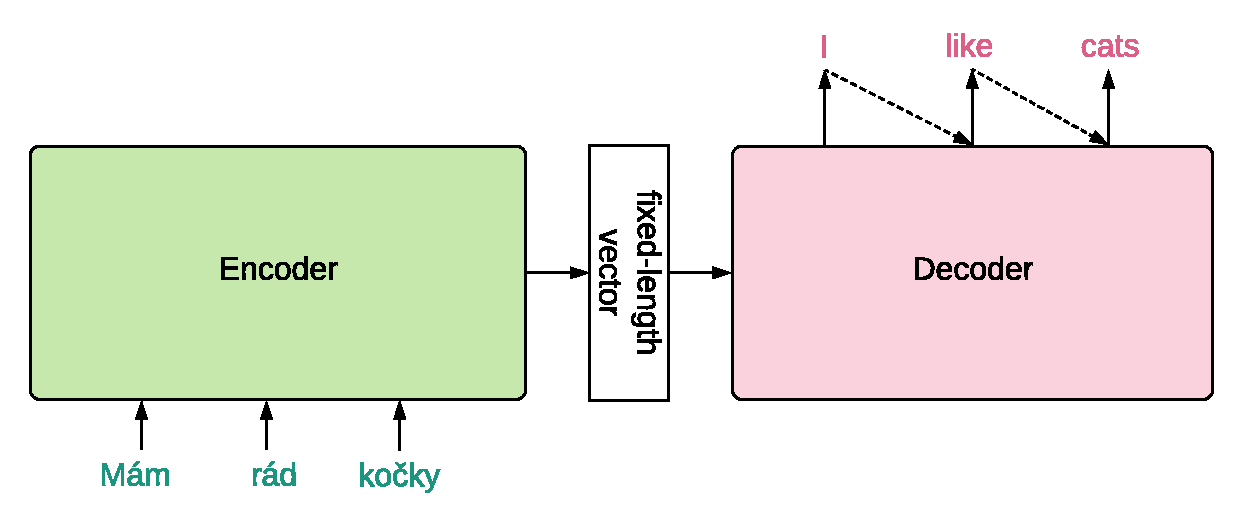
\includegraphics[width=0.6\linewidth]{img/seq2seq.pdf}
\end{figure}
\end{frame}

%------------------------------------------------

\begin{frame}{\seq2seq with attention mechanism \citep{bahdanau:etal:attention:iclr:2015,DBLP:conf/emnlp/LuongPM15}}
\begin{figure}[t]
    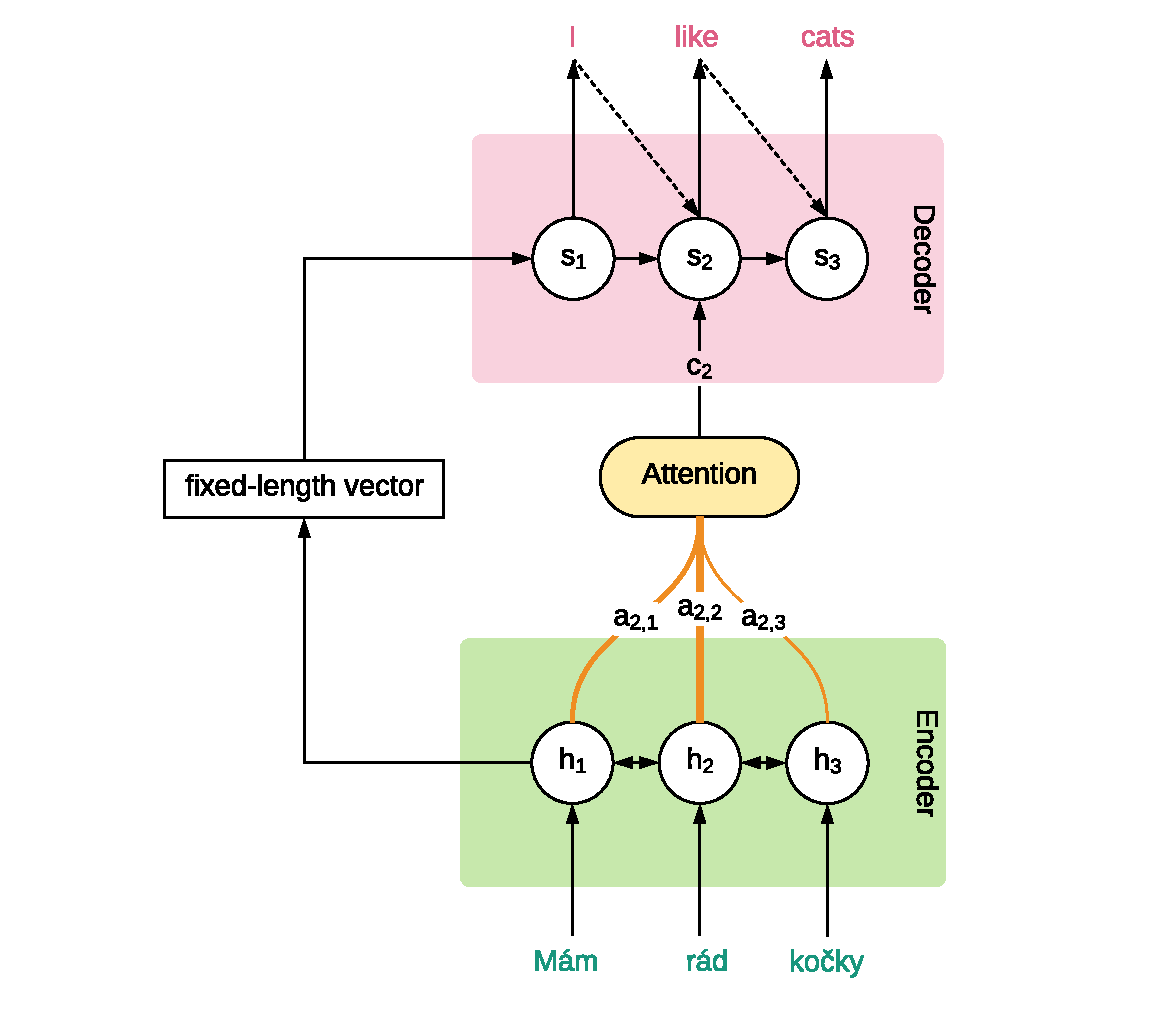
\includegraphics[width=0.6\linewidth]{img/seq2seq-att.pdf}
\end{figure}
\end{frame}

%------------------------------------------------

\begin{frame}{Attention is all you need \citep{DBLP:conf/nips/VaswaniSPUJGKP17}}
\begin{figure}[t]
    \centering
    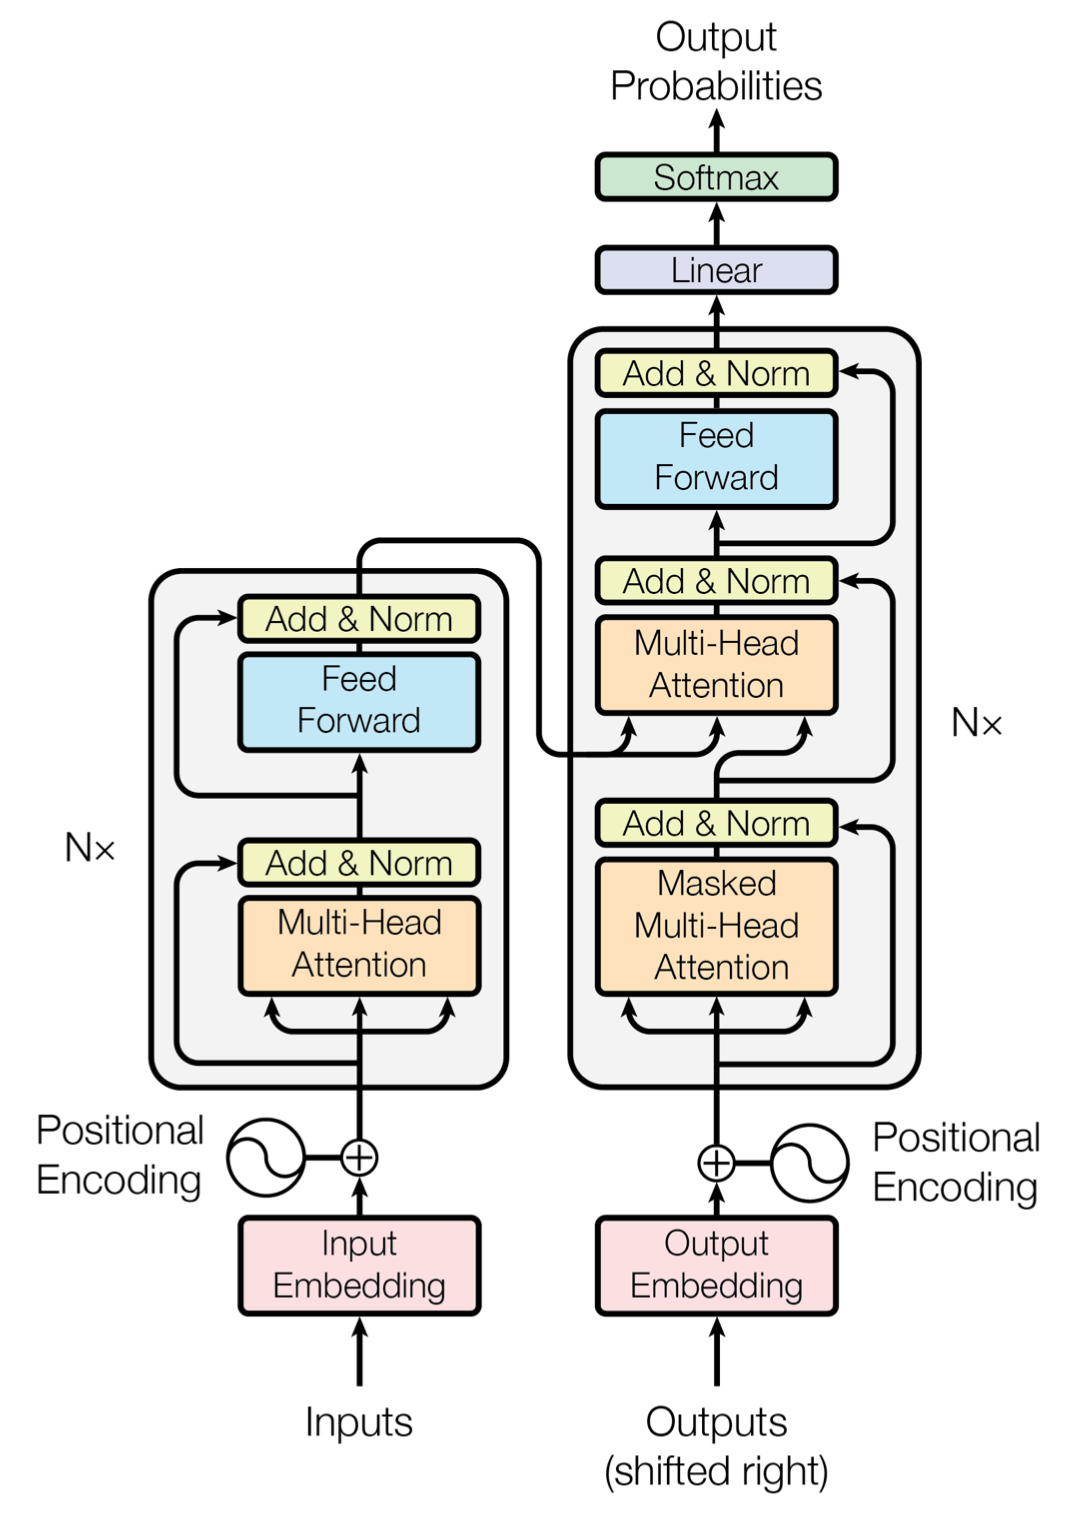
\includegraphics[width=0.5\linewidth]{img/transformer.png}
\end{figure}
\end{frame}

%------------------------------------------------

\begin{frame}{Self-Attention \citep{cheng-dong-lapata:2016:EMNLP2016}}
    \begin{figure}[t]
    \centering
    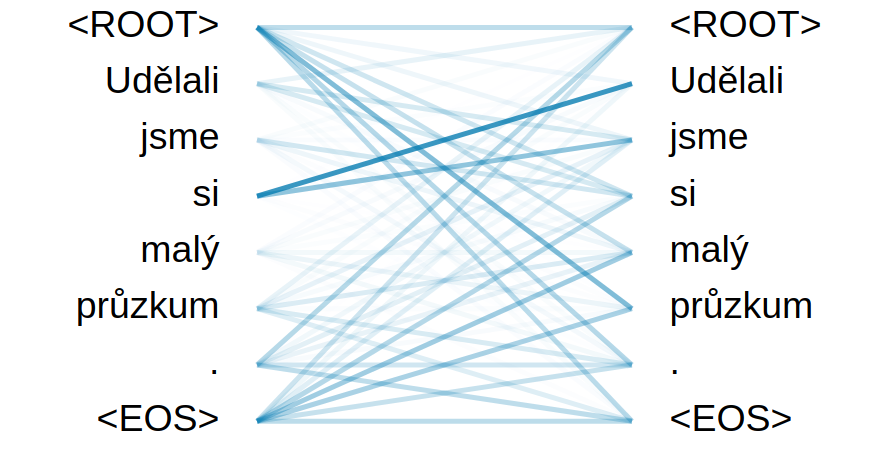
\includegraphics[width=0.6\linewidth]{img/self-att-sample.png}
    \end{figure}
\end{frame}

%------------------------------------------------

\begin{frame}{Multi-Head Attention}
    \begin{figure}[t]
    \centering
    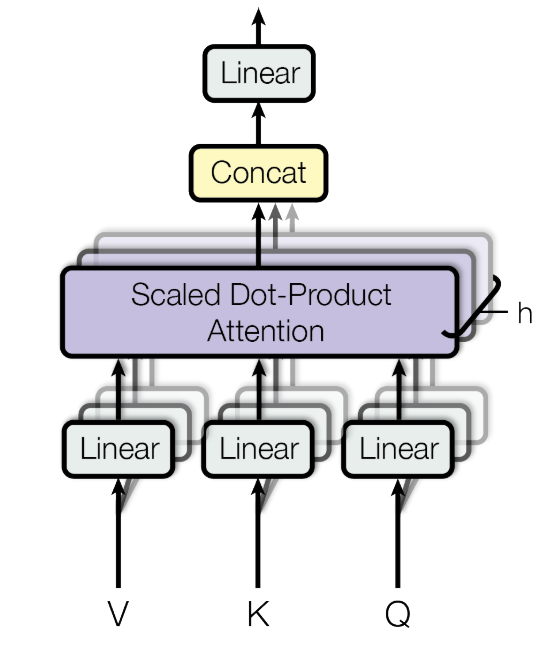
\includegraphics[width=0.5\linewidth]{img/multihead-attention.png}
    \end{figure}
\end{frame}

%------------------------------------------------

\begin{frame}{Attention Behaviors}
\begin{block}
"...the attention heads exhibit behaviour that seems related to the structure of the sentence...
\end{block}
\begin{block}
"...involved in anaphora resolution...
\end{block}
\end{frame}

%------------------------------------------------

\begin{frame}{Literature Review - Enriching NMT with Linguistic Information}
\begin{itemize}
    \item \cite{sennrich2016linguistic} reused \seq2seq model but replaced the input with the concatenation of word embeddings and linguistic features including lemmas, subword tags, POS tags and dependency labels.
    \item \cite{DBLP:conf/acl/EriguchiHT16} combined a sequence-based encoder with a tree-based encoder using Tree-LSTM \citep{DBLP:conf/acl/TaiSM15}.
    \item \cite{DBLP:conf/naacl/CohnHVYDH16} introduced structural biases to the encoder-decoder attention function.
    \item \cite{DBLP:journals/corr/abs-1711-04231} replaced Luong's global attention with their syntax-directed attention.
    \item \cite{DBLP:conf/acl/LiXTZZZ17} proposed to incorporate a sequence of structural label (POS tags) to the encoder's attention by feeding these tags to an RNN.
\end{itemize}
\end{frame}

%------------------------------------------------

\begin{frame}{Literature Review - Multi-Tasking}
\begin{itemize}
    \item \citet{DBLP:conf/acl/EriguchiTC17} combined the translation and dependency parsing tasks by sharing the translation encoder hidden states with the buffer hidden states in a shift-reduce parsing model \cite{DBLP:conf/naacl/DyerKBS16}.
    \item \citet{DBLP:conf/acl/AharoniG17a} represented the target sentence as a linearized, lexicalized constituency tree.
    \item \citet{DBLP:conf/ijcnlp/LeMYM17} made use of the same trick on dependency trees.
     \item \cite{tran2018inducing} used two different components in the encoder, one to produce the content and the other to produce the dependency matrix, then fed both to the decoder.
\end{itemize}
\end{frame}

%------------------------------------------------

\begin{frame}{Dependency Parser as Head Selection \citep{dozat:biaffine:2017}}
\begin{figure}[t]
    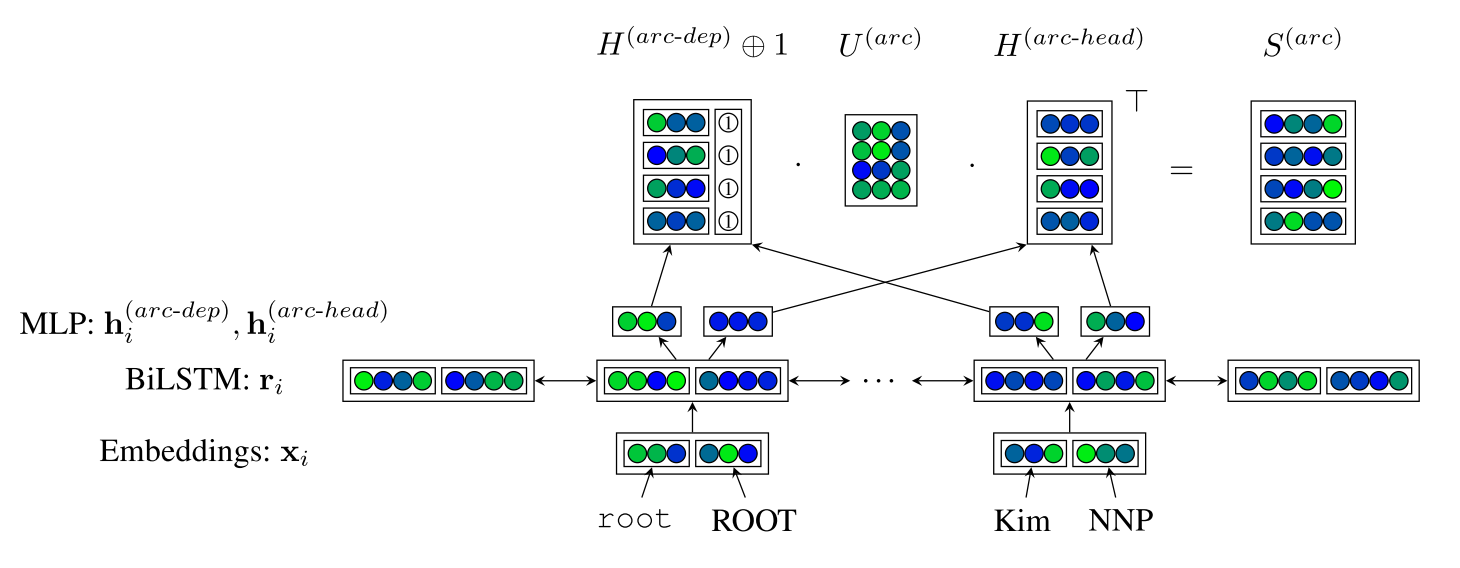
\includegraphics[width=\textwidth]{img/biaffine-parser.png}
    % \caption{Neural dependency parser with deep biaffine attention (adapted from \cite{dozat:biaffine:2017})}
    % \label{fig:biaffine-parser}
\end{figure}
\end{frame}

%------------------------------------------------

\begin{frame}{Data}
\begin{table}[t]
\small
\begin{center}
\begin{tabular}{lrr}
	& \textbf{de2cs} & \textbf{cs2en} \\
\hline
Train set sentence pairs     		& 8.8M      	& 5.2M \\
Train set source tokens		        & 89M  		    & 61M \\
Train set target tokens		        & 78M  		    & 69M \\
Development set sent. pairs         & news 2011: 3k & 1k \\
Test set sentence pairs          	& news 2013: 3k & 10k \\
Dependency parser generating the annotations				  	& UD 2.0 & Treex \\
Gold dependency treebank     & de UD test & PDT test  \\
\end{tabular}
\end{center}
\end{table}
\end{frame}

%------------------------------------------------

\begin{frame}{Attention Analysis}
\begin{figure}[t]
    \centering
    \small
    \begin{subfigure}[b]{0.6\textwidth}
        \centering
	    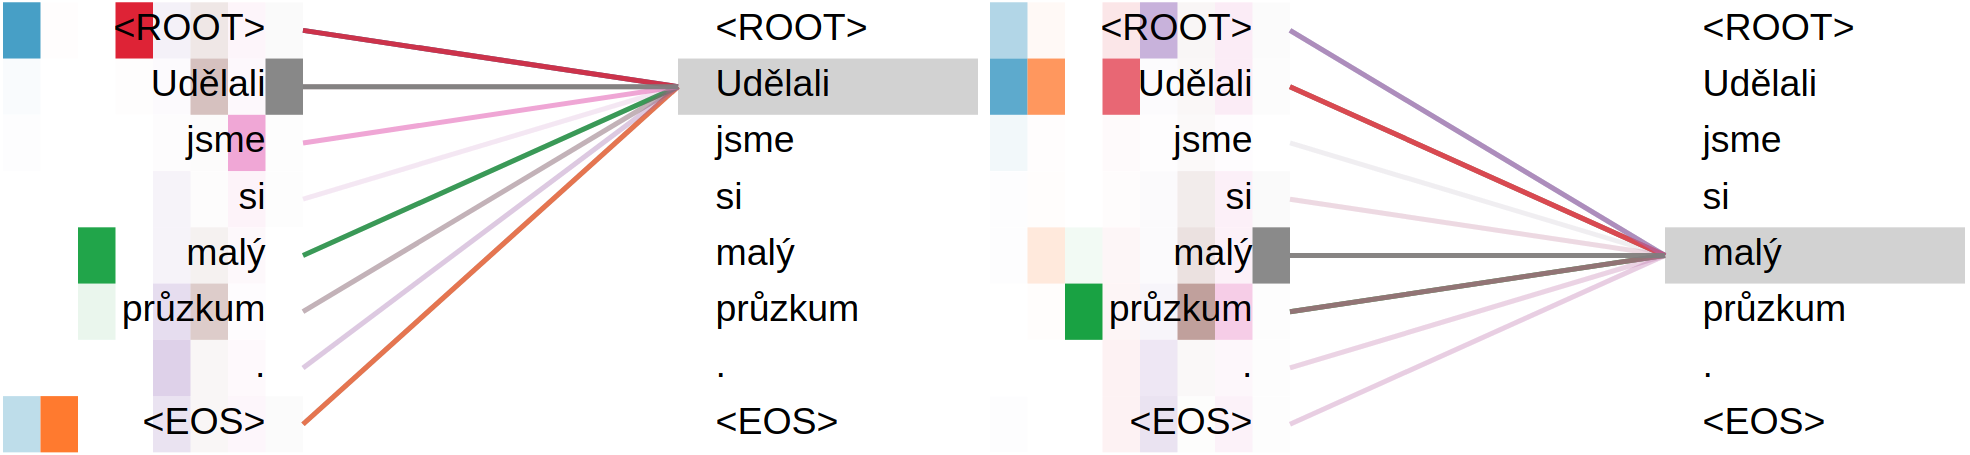
\includegraphics[width=\textwidth]{img/att-from4-l3.png}
        \caption{Layer 3}
    \end{subfigure}
    \par\medskip
    \begin{subfigure}[b]{0.6\textwidth}
        \centering
	    \frame{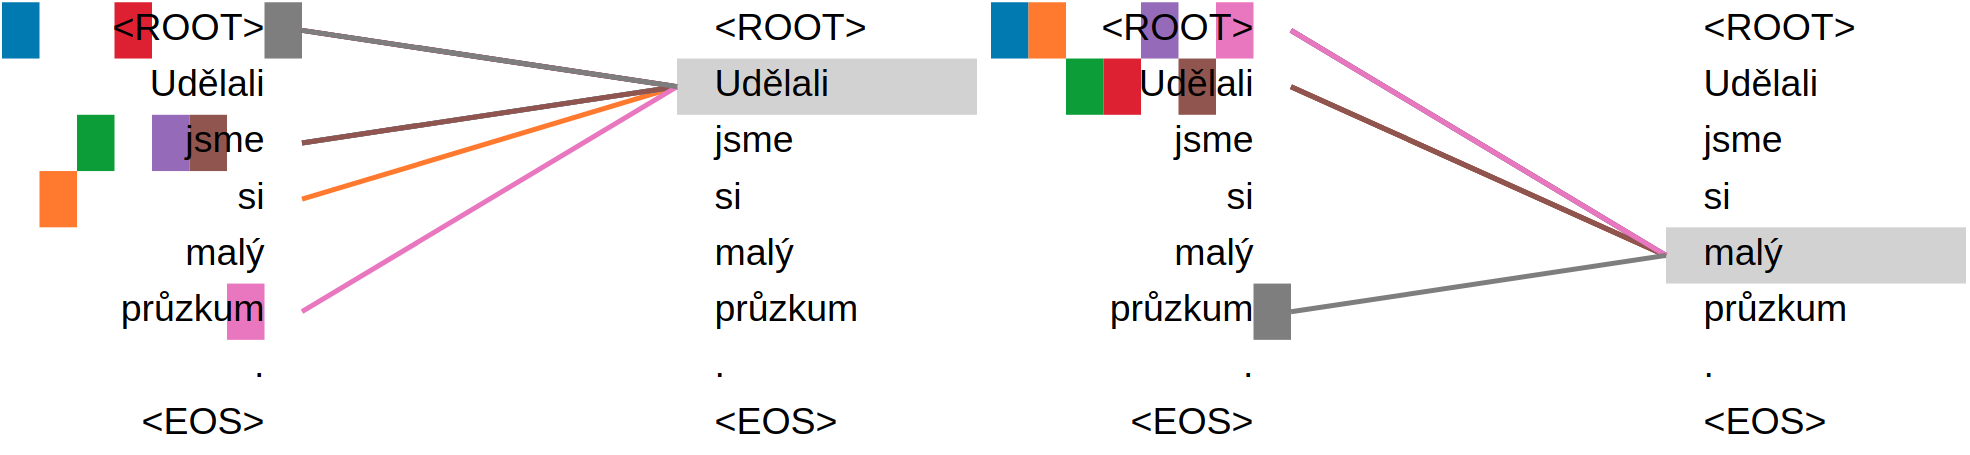
\includegraphics[width=\textwidth]{img/att-from4-l4.png}}
        \caption{Layer 4}
    \end{subfigure}
    \par\medskip
    \begin{subfigure}[b]{0.6\textwidth}
        \centering
	    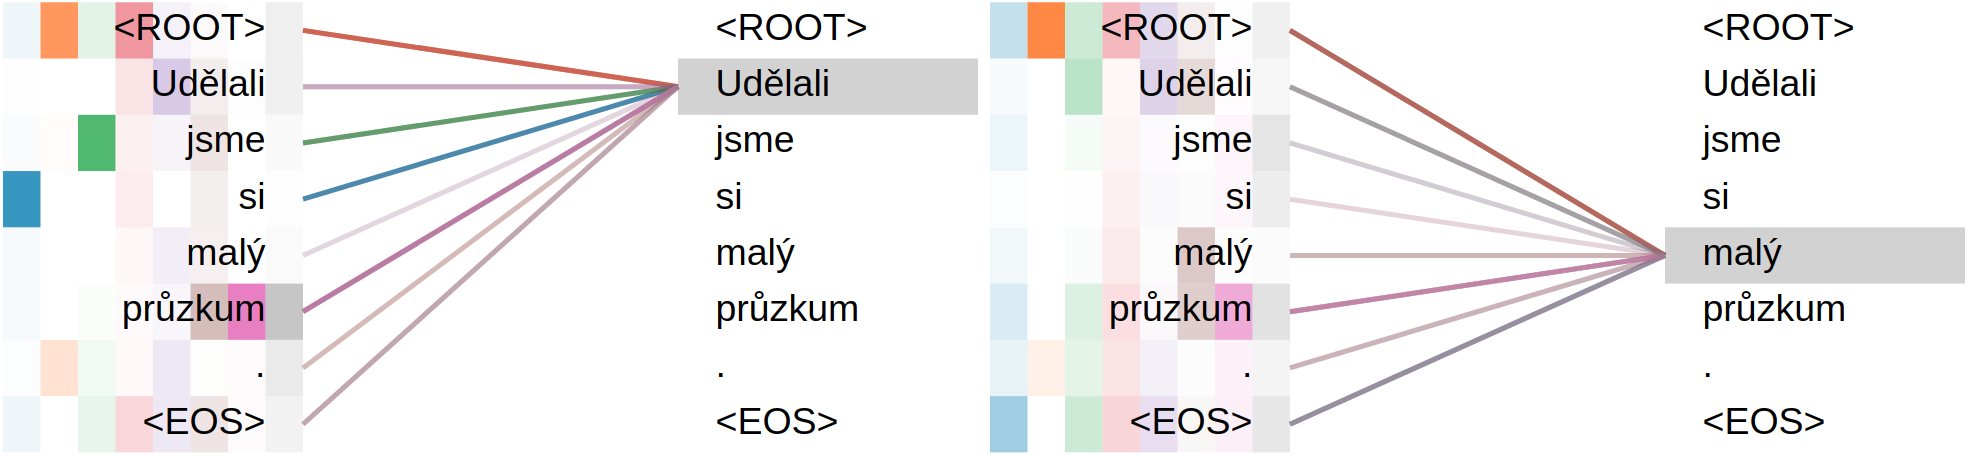
\includegraphics[width=\textwidth]{img/att-from4-l5.png}
        \caption{Layer 5}
    \end{subfigure}
    % \caption{\DepParse model with syntax demanded from the encoder's layer 4, displaying more focused attention at that layer (framed).}
\end{figure}
\end{frame}

%------------------------------------------------

\begin{frame}{Attention Analysis}
    \begin{figure}[t]
	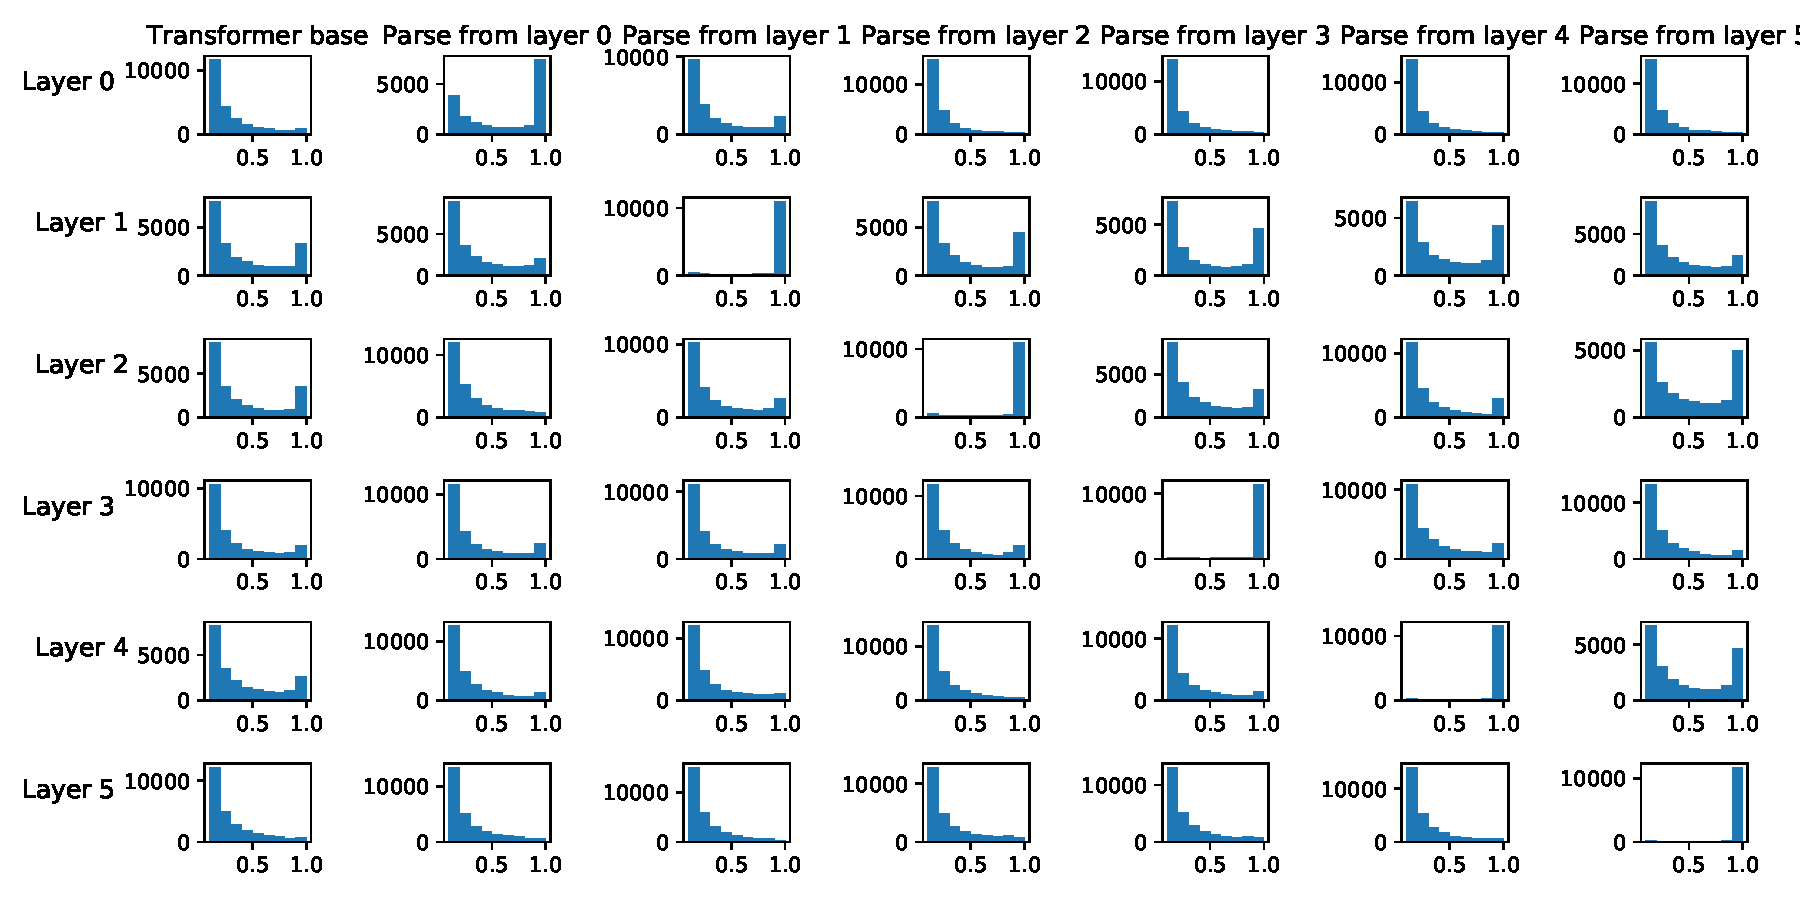
\includegraphics[width=0.75\textwidth]{img/att_dist}
    % \caption{Histogram of normalized self-attention weights for each layers (all 8 heads) in the encoder.}
    % \label{fig:att_dist}
\end{figure}
\end{frame}

%------------------------------------------------

\begin{frame}{Attention Analysis}
\begin{figure}[t]
    \centering
    \begin{subfigure}[b]{\textwidth}
	    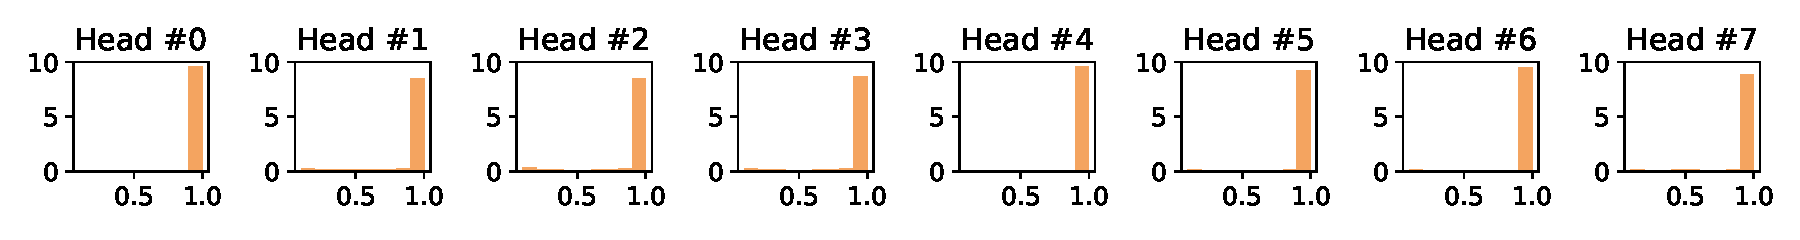
\includegraphics[width=\textwidth]{img/att_dist_4.pdf}
        \caption{\DepParse model.}
        \label{fig:att_dist_4_dep}
    \end{subfigure}
    \par\medskip
    \begin{subfigure}[b]{\textwidth}
	    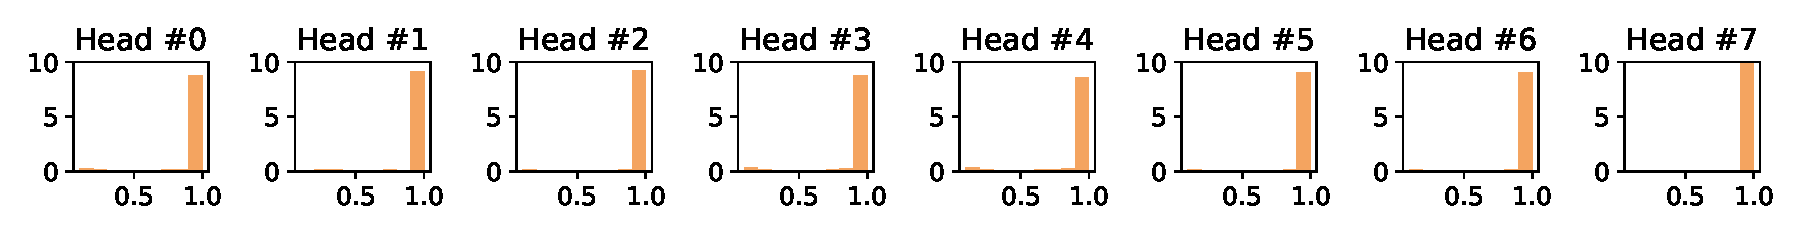
\includegraphics[width=\textwidth]{img/mono_att_dist_4.pdf}
        \caption{\DiagonalParse model.}
        \label{fig:att_dist_4_mono}
    \end{subfigure}
    % \caption{Histogram of self-attention weights for each head in layer 4 when demanding the parse tree from layer 4.}
    % \label{fig:att_dist_4}
\end{figure}
\end{frame}

%------------------------------------------------

\begin{frame}{Training Speed}
    
\begin{figure}[t]
    \centering
    \small
    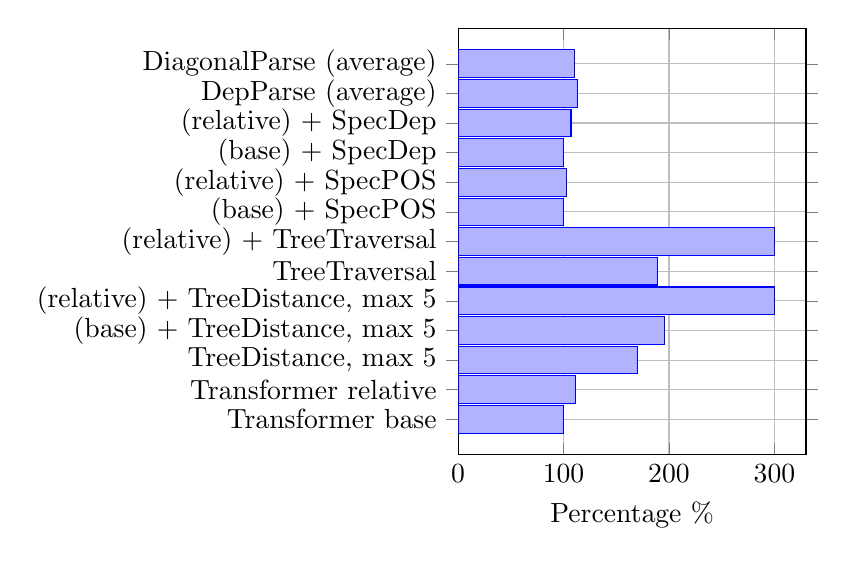
\begin{tikzpicture}
        \begin{axis}[
        height=7cm, width=6cm, grid=major,
        xbar, xmin=0,
        xlabel={Percentage \%},
        symbolic y coords={
            {Transformer base},
            {Transformer relative},
            {TreeDistance, max 5},
            {(base) + TreeDistance, max 5},
            {(relative) + TreeDistance, max 5},
            {TreeTraversal},
            {(relative) + TreeTraversal},
            {(base) + SpecPOS},
            {(relative) + SpecPOS},
            {(base) + SpecDep},
            {(relative) + SpecDep},
            {DepParse (average)},
            {DiagonalParse (average)}
        },
        ytick=data,
        % nodes near coords, nodes near coords align={horizontal},
        ytick=data,
        ]
        \addplot coordinates {
            (100,{Transformer base})
            (111,{Transformer relative})
            (170,{TreeDistance, max 5})
            (196,{(base) + TreeDistance, max 5})
            (300,{(relative) + TreeDistance, max 5})
            (189,{TreeTraversal})
            (300,{(relative) + TreeTraversal})
            (100,{(base) + SpecPOS})
            (103,{(relative) + SpecPOS})
            (100,{(base) + SpecDep})
            (107,{(relative) + SpecDep})
            (113,{DepParse (average)})
            (110,{DiagonalParse (average)})
        };
        \end{axis}
    \end{tikzpicture}
    % \caption{Training time to reach 250,000 steps on a single GPU NVIDIA GTX 1080 Ti (relative to \transformerbase).}
    % \label{fig:training-speed}
\end{figure}

\end{frame}

%----------------------------------------------------------------------------------------

\end{document}